\documentclass[12pt]{jarticle}
\usepackage{TUSIreport}
\usepackage{otf}
\usepackage[dvipdfmx]{graphicx}
\usepackage[dvipdfmx]{color}
\usepackage{amsmath}
\usepackage{amssymb}
\usepackage{color}
\usepackage{hhline}
\usepackage{fancybox,ascmac}
\usepackage{multirow}
\usepackage{url}
\usepackage{bm}
\usepackage{listings,jlisting}
%%%%%%%%%%%%%%%%%%
\lstdefinestyle{py}{
    language={Python},
    backgroundcolor={\color[gray]{.85}},
    basicstyle={\small},
    identifierstyle={\small},
    commentstyle={\small\ttfamily \color[rgb]{0,0.5,0}},
    keywordstyle={\small\bfseries \color[rgb]{1,0,0}},
    ndkeywordstyle={\small},
    stringstyle={\small\ttfamily \color[rgb]{0,0,1}},
    frame={tb},
    breaklines=true,
    columns=[l]{fullflexible},
    numbers=left,
    xrightmargin=0zw,
    xleftmargin=3zw,
    numberstyle={\scriptsize},
    stepnumber=1,
    numbersep=1zw,
    morecomment=[l]{//}
}
\begin{document}
%%%%%%%%%%%%%%%%%%%%%%%%%%%%%%%%%%%%%%%%%%%%%%%%%%%%%%%%
% 表紙を出力する場合は,\提出者と\共同実験者をいれる
% \提出者{科目名}{課題名}{提出年}{提出月}{提出日}{学籍番号}{氏名}
% \共同実験者{一人目}{二人目}{..}{..}{..}{..}{..}{八人目}
%%%%%%%%%%%%%%%%%%%%%%%%%%%%%%%%%%%%%%%%%%%%%%%%%%%%%%%
\提出者{情報工学実験3}{課題1 複雑ネットワーク入門}
{2021}{5}{27}{4619055}{辰川力駆}
%%%%%%%%%%%%%%%%%%%%%%%%%%%%%%%%%%%%%%%%%%%%%%%%%%%%%%%%%
\共同実験者{}{}{}{}{}{}{}{}
%%%%%%%%%%%%%%%%%%%%%%%%%%%%%%%%%%%%%%%%%%%%%%%%%%%%%%%%%
% 表紙を出力する場合はコメントアウトしない
%%%%%%%%%%%%%%%%%%%%%%%%%%%%%%%%%%%%%%%%%%%%%%%%%%%%%%%%%
\表紙出力
%%%%%%%%%%%%%%%%%%%%%%%%%%%%%%%%%%%%%%%%%%%%%%%%%%%%%%%
% 以下はレポート本体,reportmain.tex に書いてある.
% \inputを使っているが,直接書いても良い.
%%%%%%%%%%%%%%%%%%%%%%%%%%%%%%%%%%%%%%%%%%%%%%%%%%%%%%%
\section{実験内容}
\subsection{課題1}
次のネットワーク例において、何が頂点で何が枝かを考える。
また、このネットワーク例以外で実世界におけるネットワークの例を考える。
\begin{enumerate}
    \item インターネット
    \item WWW
    \item 神経回路網
    \item 航空網、鉄道網、道路網
    \item 電力輸送網
\end{enumerate}

\subsection{課題2}
\begin{enumerate}
    \item 図1に示したネットワークの隣接行列を求める。
    \item 図2に示したネットワークの隣接行列を求める。
\end{enumerate}
\begin{figure}[h]
    \begin{center}
        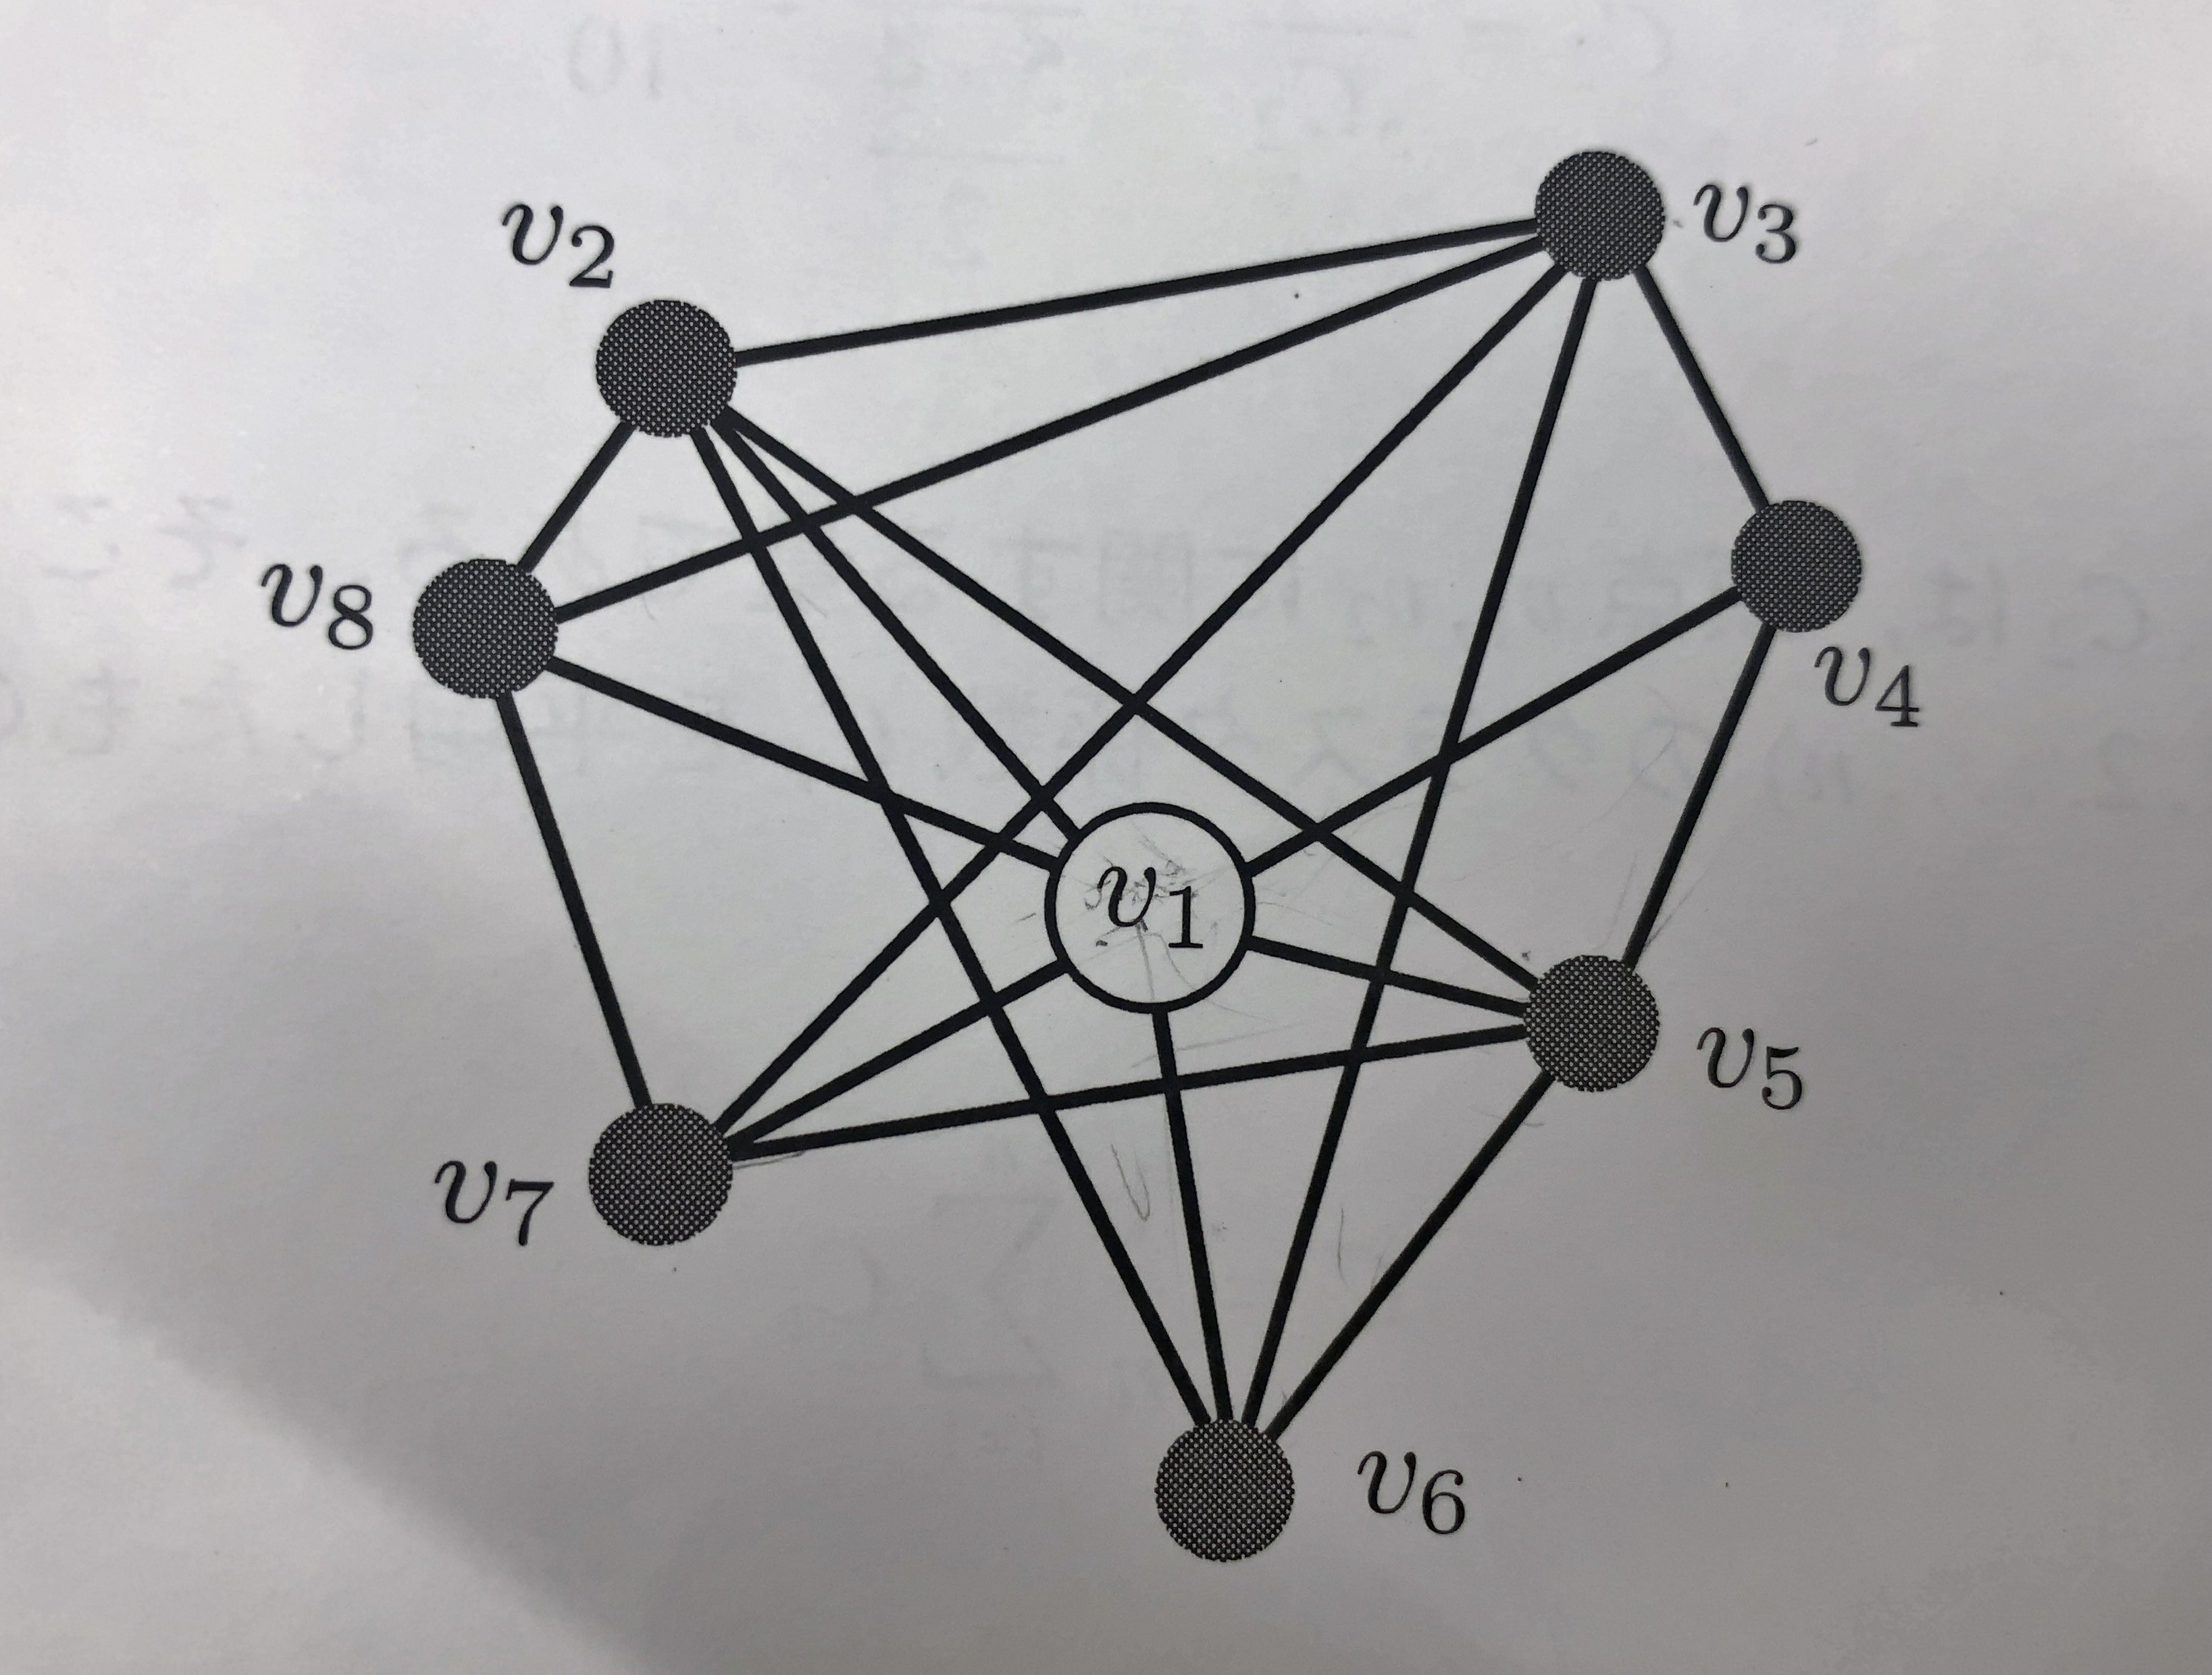
\includegraphics[scale=0.1]{kadai1_1.jpg}
    \end{center}
    \caption{ネットワーク例1}
\end{figure}

\clearpage
\begin{figure}[h]
    \begin{center}
        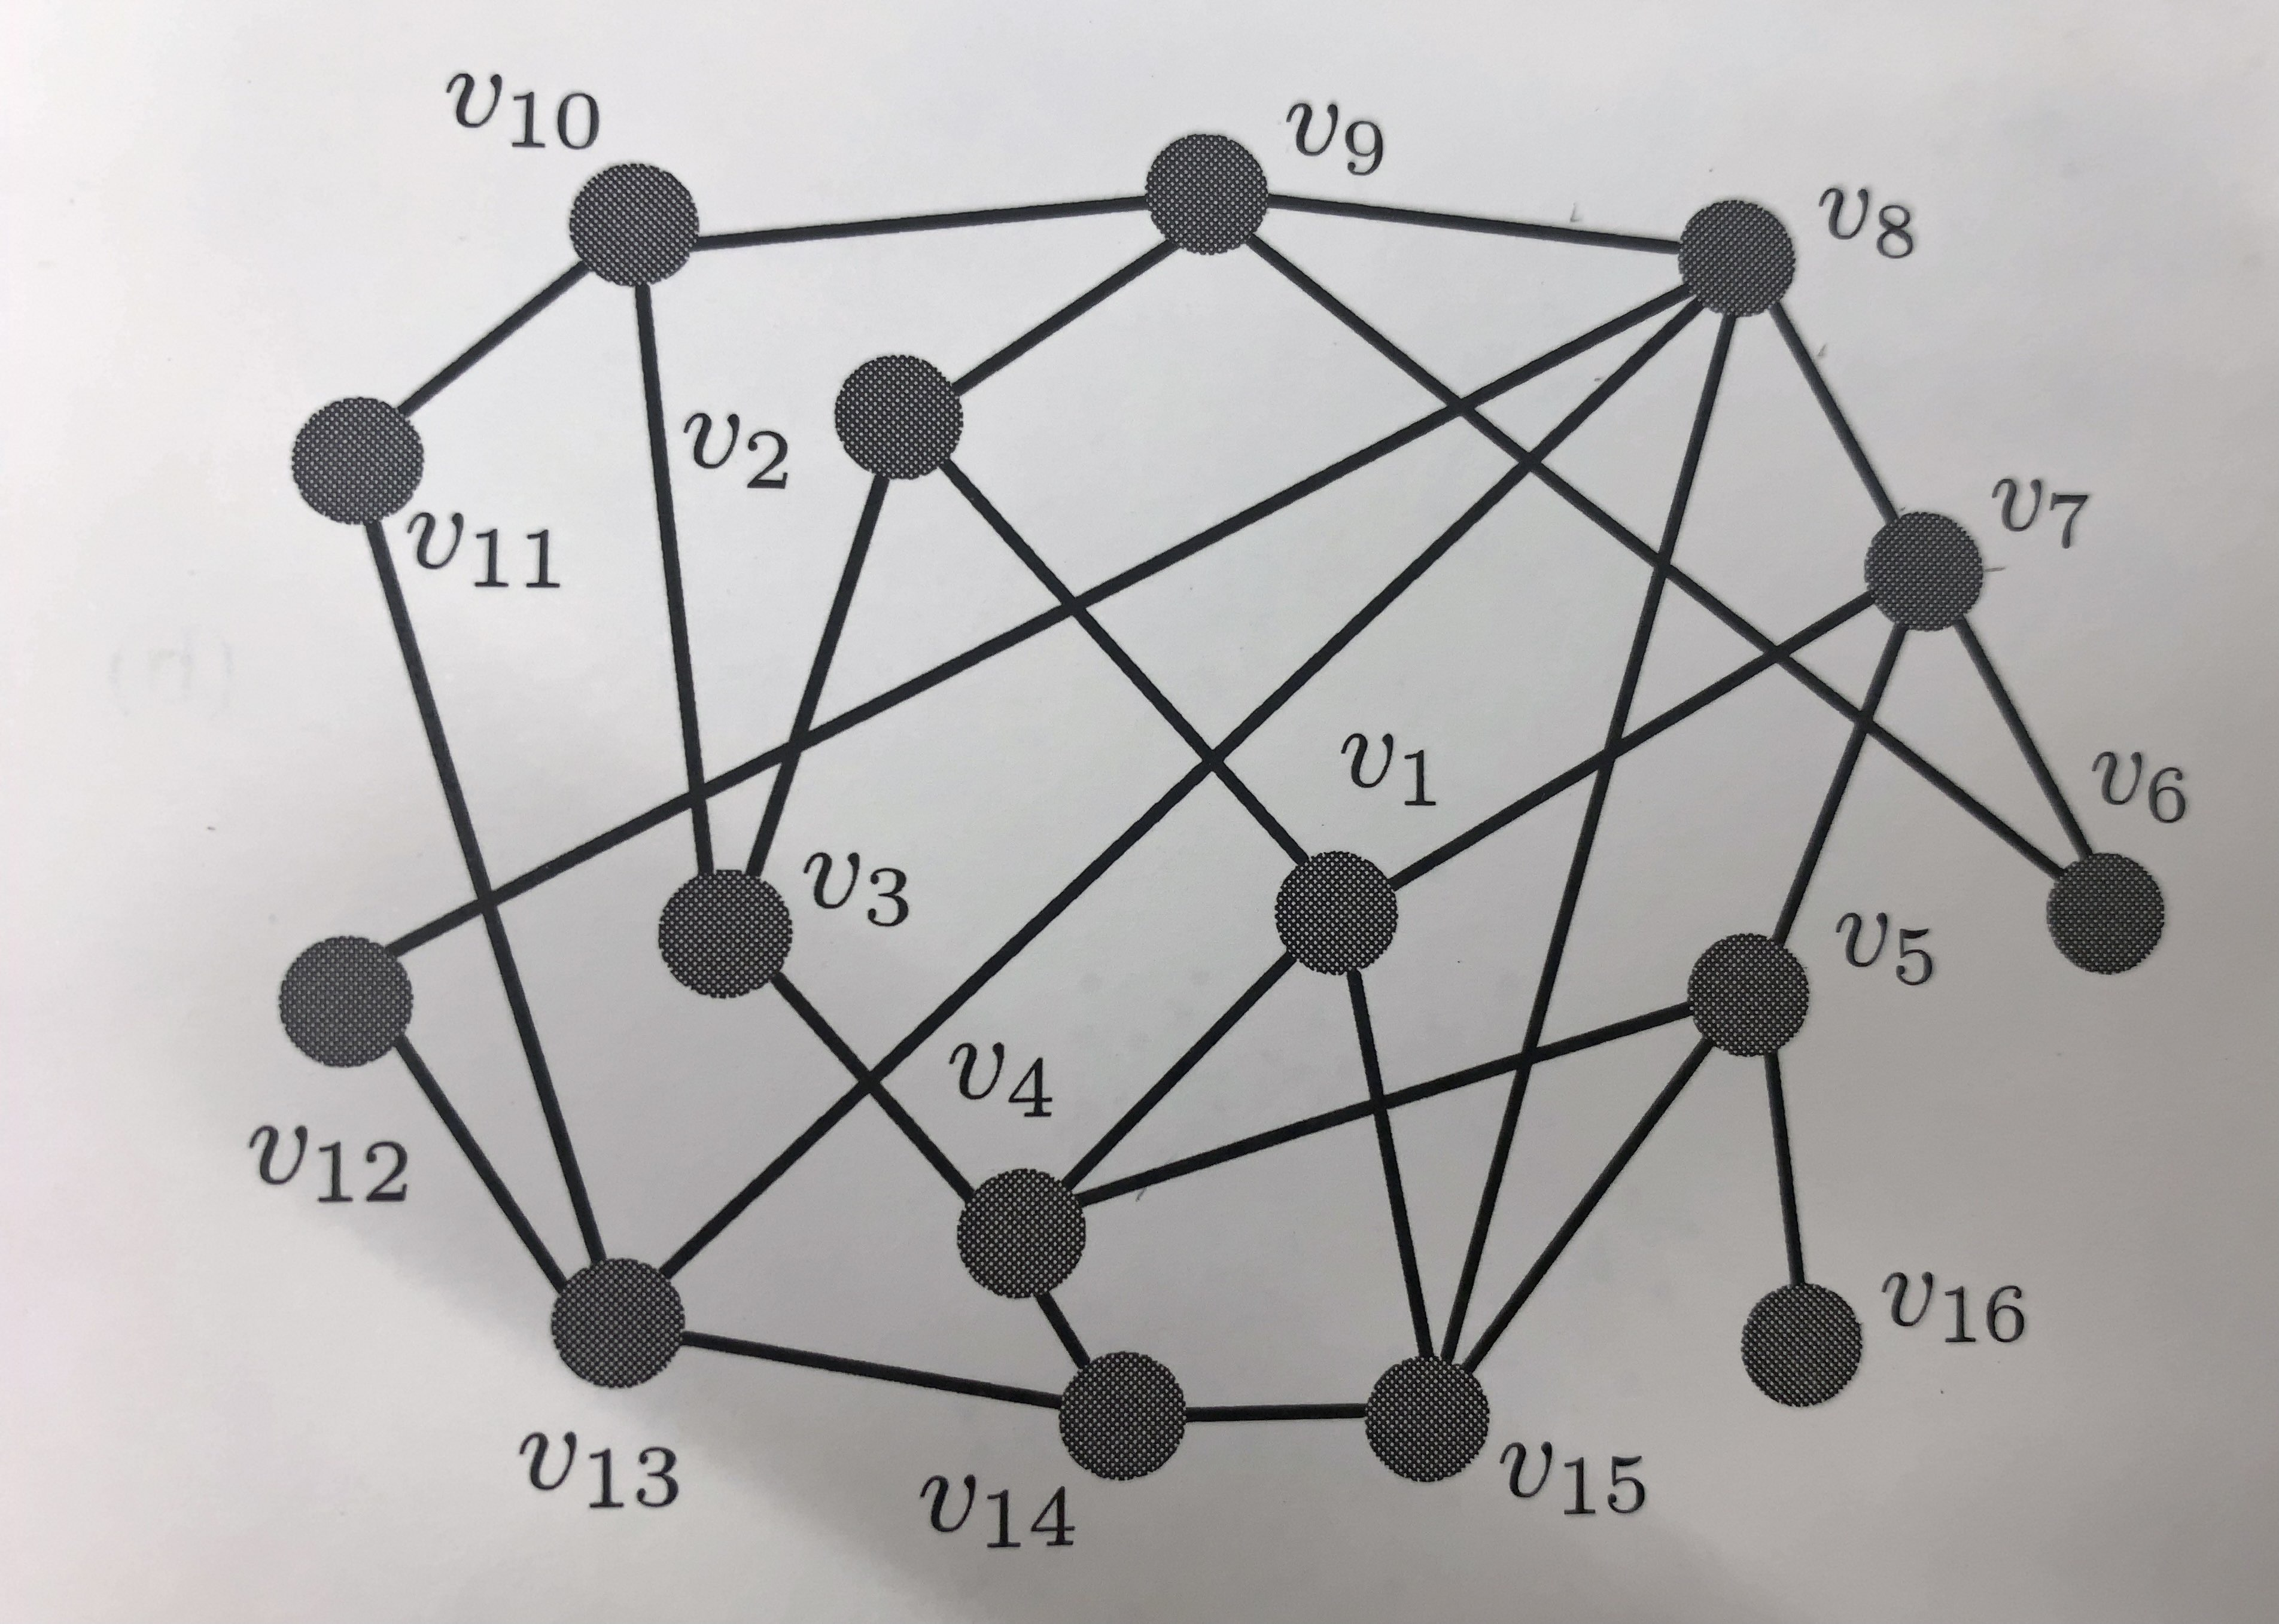
\includegraphics[scale=0.1]{kadai1_2.jpg}
    \end{center}
    \caption{ネットワーク例2}
\end{figure}

\subsection{課題3}
\begin{enumerate}
    \item 図1に示したネットワークの隣接リストを求める。
    \item 図2に示したネットワークの隣接リストを求める。
\end{enumerate}

\subsection{課題4}
\begin{enumerate}
    \item 図1に示したネットワークの次数分布を求める。
    \item 図2に示したネットワークの次数分布を求める。
\end{enumerate}

\subsection{課題5}
\begin{enumerate}
    \item 図1のネットワークにおいて、$C_i(i=3,4,...,8)$を求める。
    \item 図1のネットワークのクラスタ係数$C$を求める。
\end{enumerate}

\subsection{課題6}
\begin{enumerate}
    \item 図2のネットワークにおいて、$d_{i,j}(i,j=1,2,...,16)$を求める。
    \item 図2のネットワークにおいて、平均頂点間距離$L$を求める。
\end{enumerate}

\clearpage

\subsection{課題7}
\begin{enumerate}
    \item あるネットワークに対して、平均頂点間距離、クラスタ係数を求めるコードを作成する。
          ただし、本実験でのネットワークデータは、枝リスト形式で与えられているとする。
    \item 1で作成したコードを用いて、次の3つのネットワークの平均頂点間距離とクラスタ係数を求める。
          \begin{enumerate}
              \item Zacharyの空手クラブの友人関係
              \item イルカのネットワーク
              \item 線虫の神経回路網
          \end{enumerate}
    \item 上記の3つのネットワークについて、各々をランダマイズしたネットワークを作成し、
          それらの平均頂点間距離、クラスタ係数を求め、元のネットワークの平均頂点間距離、クラスタ係数と比較する。
\end{enumerate}

\section{実験結果}
\subsection{課題1}
\begin{table}[htb]
    \caption{現実のネットワーク例}
    \begin{center}
        \begin{tabular}{|c||c|c|}
            \hline
                                   & 頂点           & 枝             \\ \hline \hline
            インターネット         & コンピュータ   & 回線           \\ \hline
            WWW                    & ウェブサイト   & ハイパーリンク \\ \hline
            神経回路網             & 神経細胞       & シナプス       \\ \hline
            航空網、鉄道網、道路網 & 空港、駅、建物 & 路線、線路、道 \\ \hline
            電力輸送網             & 建物           & 電線           \\ \hline
            人間の交友関係         & 人             & 人間関係       \\ \hline
        \end{tabular}
    \end{center}
\end{table}

\subsection{課題2}
図1のネットワークの隣接行列を$A$、図2のネットワークの隣接行列を$B$とすると、次のようになる。

\begin{center}
    \(
    A = \left(
    \begin{array}{cccccccc}
        0 & 1 & 0 & 1 & 1 & 1 & 1 & 1 \\
        1 & 0 & 1 & 0 & 1 & 1 & 0 & 1 \\
        0 & 1 & 0 & 1 & 0 & 1 & 1 & 1 \\
        1 & 0 & 1 & 0 & 1 & 0 & 0 & 0 \\
        1 & 1 & 0 & 1 & 0 & 1 & 1 & 0 \\
        1 & 1 & 1 & 0 & 1 & 0 & 0 & 0 \\
        1 & 0 & 1 & 0 & 1 & 0 & 0 & 1 \\
        1 & 1 & 1 & 0 & 0 & 0 & 1 & 0
    \end{array}
    \right)
    \)
\end{center}

\clearpage
\begin{center}
    \(
    B = \left(
    \begin{array}{cccccccccccccccc}
        0 & 1 & 0 & 1 & 0 & 0 & 1 & 0 & 0 & 0 & 0 & 0 & 0 & 0 & 1 & 0 \\
        1 & 0 & 1 & 0 & 0 & 0 & 0 & 0 & 1 & 0 & 0 & 0 & 0 & 0 & 0 & 0 \\
        0 & 1 & 0 & 1 & 0 & 0 & 0 & 0 & 0 & 1 & 0 & 0 & 0 & 0 & 0 & 0 \\
        1 & 0 & 1 & 0 & 1 & 0 & 0 & 0 & 0 & 0 & 0 & 0 & 0 & 1 & 0 & 0 \\
        0 & 0 & 0 & 1 & 0 & 0 & 1 & 0 & 0 & 0 & 0 & 0 & 0 & 0 & 1 & 1 \\
        0 & 0 & 0 & 0 & 0 & 0 & 1 & 0 & 1 & 0 & 0 & 0 & 0 & 0 & 0 & 0 \\
        1 & 0 & 0 & 0 & 1 & 1 & 0 & 1 & 0 & 0 & 0 & 0 & 0 & 0 & 0 & 0 \\
        0 & 0 & 0 & 0 & 0 & 0 & 1 & 0 & 1 & 0 & 0 & 1 & 1 & 0 & 1 & 0 \\
        0 & 1 & 0 & 0 & 0 & 1 & 0 & 1 & 0 & 1 & 0 & 0 & 0 & 0 & 0 & 0 \\
        0 & 0 & 1 & 0 & 0 & 0 & 0 & 0 & 1 & 0 & 1 & 0 & 0 & 0 & 0 & 0 \\
        0 & 0 & 0 & 0 & 0 & 0 & 0 & 0 & 0 & 1 & 0 & 0 & 1 & 0 & 0 & 0 \\
        0 & 0 & 0 & 0 & 0 & 0 & 0 & 1 & 0 & 0 & 0 & 0 & 1 & 0 & 0 & 0 \\
        0 & 0 & 0 & 0 & 0 & 0 & 0 & 1 & 0 & 0 & 1 & 1 & 0 & 1 & 0 & 0 \\
        0 & 0 & 0 & 1 & 0 & 0 & 0 & 0 & 0 & 0 & 0 & 0 & 1 & 0 & 1 & 0 \\
        1 & 0 & 0 & 0 & 1 & 0 & 0 & 1 & 0 & 0 & 0 & 0 & 0 & 1 & 0 & 0 \\
        0 & 0 & 0 & 0 & 1 & 0 & 0 & 0 & 0 & 0 & 0 & 0 & 0 & 0 & 0 & 0
    \end{array}
    \right)
    \)
\end{center}

\subsection{課題3}
\begin{table}[htb]
    \caption{図1のネットワークの隣接リスト}
    \begin{center}
        \begin{tabular}{|c|l|}
            \hline
            頂点番号 & 接続先の頂点番号 \\ \hline \hline
            1        & 2,4,5,6,7,8      \\ \hline
            2        & 1,3,5,6,8        \\ \hline
            3        & 2,4,6,7,8        \\ \hline
            4        & 1,3,5            \\ \hline
            5        & 1,2,4,6,7        \\ \hline
            6        & 1,2,3,5          \\ \hline
            7        & 1,3,5,8          \\ \hline
            8        & 1,2,3,7          \\ \hline
        \end{tabular}
    \end{center}
\end{table}

\clearpage

\begin{table}[htb]
    \caption{図2のネットワークの隣接リスト}
    \begin{center}
        \begin{tabular}{|c|l|}
            \hline
            頂点番号 & 接続先の頂点番号 \\ \hline \hline
            1        & 2,4,7,15         \\ \hline
            2        & 1,3,9            \\ \hline
            3        & 2,4,10           \\ \hline
            4        & 1,3,5,14         \\ \hline
            5        & 4,7,15,16        \\ \hline
            6        & 7,9              \\ \hline
            7        & 1,5,6,8          \\ \hline
            8        & 7,9,12,13,15     \\ \hline
            9        & 2,6,8,10         \\ \hline
            10       & 3,9,11           \\ \hline
            11       & 10,13            \\ \hline
            12       & 8,13             \\ \hline
            13       & 8,11,12,14       \\ \hline
            14       & 4,13,15          \\ \hline
            15       & 1,5,8,14         \\ \hline
            16       & 5                \\ \hline
        \end{tabular}
    \end{center}
\end{table}

\subsection{課題4}
\begin{enumerate}
    \item 図1に示したネットワークの次数分布は、表2より、
          \begin{eqnarray*}
              p(0)=0, p(1)=0, p(2)=0, p(3)=\frac{1}{8}, p(4)=\frac{3}{8}, p(5)=\frac{3}{8}, p(6)=\frac{1}{8}, p(k)=0(k>6)
          \end{eqnarray*}
          となった。
    \item 図2に示したネットワークの次数分布は、表3より、
          \begin{eqnarray*}
              p(0)=0, p(1)=\frac{1}{16}, p(2)=\frac{3}{16}, p(3)=\frac{1}{4}, p(4)=\frac{7}{16}, p(5)=\frac{1}{16}, p(k)=0(k>5)
          \end{eqnarray*}
          となった。
\end{enumerate}

\clearpage
\subsection{課題5}
\begin{enumerate}
    \item 図1のネットワークにおいて$C_i(i=3,4,...,8)$は、
          \begin{eqnarray*}
              C_3=\frac{3}{10}, C_4=\frac{1}{3}, C_5=\frac{1}{2}, C_6=\frac{2}{3}, C_7=\frac{1}{2}, C_8=\frac{2}{3}
          \end{eqnarray*}
          である。
    \item 図1のネットワークのクラスタ係数$C$は、
          \begin{eqnarray*}
              C=\frac{1}{8} \sum_{n = 1}^{8} C_i =0.5042
          \end{eqnarray*}
          である。
\end{enumerate}

\subsection{課題6}
\begin{enumerate}
    \item 図2のネットワークにおいて、$d_{i,j}$は、
          \begin{center}
              \(
              d_{i,j} = \left(
              \begin{array}{cccccccccccccccc}
                      0 & 1 & 2 & 1 & 2 & 2 & 1 & 2 & 2 & 3 & 4 & 3 & 3 & 2 & 1 & 3 \\
                        & 0 & 1 & 2 & 3 & 2 & 2 & 2 & 1 & 2 & 3 & 3 & 3 & 3 & 2 & 4 \\
                        &   & 0 & 1 & 2 & 3 & 3 & 3 & 2 & 1 & 2 & 4 & 3 & 2 & 3 & 3 \\
                        &   &   & 0 & 1 & 3 & 2 & 3 & 3 & 2 & 3 & 3 & 2 & 1 & 2 & 2 \\
                        &   &   &   & 0 & 2 & 1 & 2 & 3 & 3 & 4 & 3 & 3 & 2 & 1 & 1 \\
                        &   &   &   &   & 0 & 1 & 2 & 1 & 2 & 3 & 3 & 3 & 4 & 3 & 3 \\
                        &   &   &   &   &   & 0 & 1 & 2 & 3 & 3 & 2 & 2 & 3 & 2 & 2 \\
                        &   &   &   &   &   &   & 0 & 1 & 2 & 2 & 1 & 1 & 2 & 1 & 3 \\
                        &   &   &   &   &   &   &   & 0 & 1 & 2 & 2 & 2 & 3 & 2 & 4 \\
                        &   &   &   &   &   &   &   &   & 0 & 1 & 3 & 2 & 3 & 3 & 4 \\
                        &   &   &   &   &   &   &   &   &   & 0 & 2 & 1 & 2 & 3 & 5 \\
                        &   &   &   &   &   &   &   &   &   &   & 0 & 1 & 2 & 2 & 4 \\
                        &   &   &   &   &   &   &   &   &   &   &   & 0 & 1 & 2 & 4 \\
                        &   &   &   &   &   &   &   &   &   &   &   &   & 0 & 1 & 3 \\
                        &   &   &   &   &   &   &   &   &   &   &   &   &   & 0 & 2 \\
                        &   &   &   &   &   &   &   &   &   &   &   &   &   &   & 0
                  \end{array}
              \right)
              \)
          \end{center}
    \item 図2のネットワークの平均頂点間距離は
          \begin{eqnarray*}
              L=\frac{1}{{}_{16} C_{2}} \sum_{i = 1}^{16} \sum_{j = 1,j>i}^{16}d_{i,j} =2.283
          \end{eqnarray*}
          である。
\end{enumerate}

\clearpage

\subsection{課題7}

\begin{enumerate}
    \item 作成したコードはzipファイルに添付した。
    \item 1で作成したコードを用いて、次の3つのネットワークの平均頂点間距離とクラスタ係数を求めると、
          表4のようになった。

          \begin{table}[htb]
              \caption{3つのネットワークの平均頂点間距離とクラスタ係数}
              \begin{center}
                  \begin{tabular}{|c||c|c|}
                      \hline
                      ネットワーク                  & $L_{\text{org}}$ & $C_{\text{org}}$ \\ \hline \hline
                      Zacharyの空手クラブの友人関係 & 2.4082           & 0.5706           \\ \hline
                      イルカのネットワーク          & 3.3570           & 0.2590           \\ \hline
                      線虫の神経回路網              & 2.4356           & 0.3371           \\ \hline
                  \end{tabular}
              \end{center}
          \end{table}
    \item 各々をランダマイズしたネットワークの平均頂点間距離、クラスタ係数は、
          表5のようになった。

          \begin{table}[htb]
              \caption{ランダマイズした3つのネットワークの平均頂点間距離とクラスタ係数}
              \begin{center}
                  \begin{tabular}{|c||c|c|}
                      \hline
                      ネットワーク                  & $\overline{L}_{R}$ & $\overline{C}_{R}$ \\ \hline \hline
                      Zacharyの空手クラブの友人関係 & 2.0926             & 0.3520             \\ \hline
                      イルカのネットワーク          & 2.3408             & 0.1161             \\ \hline
                      線虫の神経回路網              & 2.2678             & 0.1426             \\ \hline
                  \end{tabular}
              \end{center}
          \end{table}
\end{enumerate}

\clearpage
\section{考察}
配布された3つのネットワークについて、スモールワールド構造を有するかを考える。
\begin{table}[htb]
    \caption{平均頂点間距離とクラスタ係数の比}
    \begin{center}
        \begin{tabular}{|c||c|c|}
            \hline
            ネットワーク                  & $\frac{L_{\text{org}}}{\overline{L}_{R}}$ & $\frac{C_{\text{org}}}{\overline{C}_{R}}$ \\ \hline \hline
            Zacharyの空手クラブの友人関係 & 1.1508                                    & 1.6210                                    \\ \hline
            イルカのネットワーク          & 1.4341                                    & 2.2308                                    \\ \hline
            線虫の神経回路網              & 1.0740                                    & 2.3640                                    \\ \hline
        \end{tabular}
    \end{center}
\end{table}

表6より、Zacharyの空手クラブの友人関係、
イルカのネットワーク、
線虫の神経回路網
のすべてが、$\frac{L_{\text{org}}}{\overline{L}_{R}}\thickapprox 1$となった。
さらに、すべてが、$\frac{C_{\text{org}}}{\overline{C}_{R}} \gg 1$となった。

よって、これらのネットワークについて、すべてスモールワールド構造を有することが分かる。
\clearpage
\appendix

%%%%%%%%%%%%%%%%%%%%%%%%%%%%%%%%%%%%%%%%%%%%%%%%%%%%%%%
\end{document}